
%% bare_conf.tex
%% V1.3
%% 2007/01/11
%% by Michael Shell
%% See:
%% http://www.michaelshell.org/
%% for current contact information.
%%
%% This is a skeleton file demonstrating the use of IEEEtran.cls
%% (requires IEEEtran.cls version 1.7 or later) with an IEEE conference paper.
%%
%% Support sites:
%% http://www.michaelshell.org/tex/ieeetran/
%% http://www.ctan.org/tex-archive/macros/latex/contrib/IEEEtran/
%% and
%% http://www.ieee.org/

%%*************************************************************************
%% Legal Notice:
%% This code is offered as-is without any warranty either expressed or
%% implied; without even the implied warranty of MERCHANTABILITY or
%% FITNESS FOR A PARTICULAR PURPOSE! 
%% User assumes all risk.
%% In no event shall IEEE or any contributor to this code be liable for
%% any damages or losses, including, but not limited to, incidental,
%% consequential, or any other damages, resulting from the use or misuse
%% of any information contained here.
%%
%% All comments are the opinions of their respective authors and are not
%% necessarily endorsed by the IEEE.
%%
%% This work is distributed under the LaTeX Project Public License (LPPL)
%% ( http://www.latex-project.org/ ) version 1.3, and may be freely used,
%% distributed and modified. A copy of the LPPL, version 1.3, is included
%% in the base LaTeX documentation of all distributions of LaTeX released
%% 2003/12/01 or later.
%% Retain all contribution notices and credits.
%% ** Modified files should be clearly indicated as such, including  **
%% ** renaming them and changing author support contact information. **
%%
%% File list of work: IEEEtran.cls, IEEEtran_HOWTO.pdf, bare_adv.tex,
%%                    bare_conf.tex, bare_jrnl.tex, bare_jrnl_compsoc.tex
%%*************************************************************************

% *** Authors should verify (and, if needed, correct) their LaTeX system  ***
% *** with the testflow diagnostic prior to trusting their LaTeX platform ***
% *** with production work. IEEE's font choices can trigger bugs that do  ***
% *** not appear when using other class files.                            ***
% The testflow support page is at:
% http://www.michaelshell.org/tex/testflow/



% Note that the a4paper option is mainly intended so that authors in
% countries using A4 can easily print to A4 and see how their papers will
% look in print - the typesetting of the document will not typically be
% affected with changes in paper size (but the bottom and side margins will).
% Use the testflow package mentioned above to verify correct handling of
% both paper sizes by the user's LaTeX system.
%
% Also note that the "draftcls" or "draftclsnofoot", not "draft", option
% should be used if it is desired that the figures are to be displayed in
% draft mode.
%
\documentclass[conference]{IEEEtran}
% Add the compsoc option for Computer Society conferences.
%
% If IEEEtran.cls has not been installed into the LaTeX system files,
% manually specify the path to it like:
% \documentclass[conference]{../sty/IEEEtran}

% Some very useful LaTeX packages include:
% (uncomment the ones you want to load)
%
% *** MISC UTILITY PACKAGES ***
%
%\usepackage{ifpdf}
% Heiko Oberdiek's ifpdf.sty is very useful if you need conditional
% compilation based on whether the output is pdf or dvi.
% usage:
% \ifpdf
%   % pdf code
% \else
%   % dvi code
% \fi
% The latest version of ifpdf.sty can be obtained from:
% http://www.ctan.org/tex-archive/macros/latex/contrib/oberdiek/
% Also, note that IEEEtran.cls V1.7 and later provides a builtin
% \ifCLASSINFOpdf conditional that works the same way.
% When switching from latex to pdflatex and vice-versa, the compiler may
% have to be run twice to clear warning/error messages.






% *** CITATION PACKAGES ***
%
%\usepackage{cite}
% cite.sty was written by Donald Arseneau
% V1.6 and later of IEEEtran pre-defines the format of the cite.sty package
% \cite{} output to follow that of IEEE. Loading the cite package will
% result in citation numbers being automatically sorted and properly
% "compressed/ranged". e.g., [1], [9], [2], [7], [5], [6] without using
% cite.sty will become [1], [2], [5]--[7], [9] using cite.sty. cite.sty's
% \cite will automatically add leading space, if needed. Use cite.sty's
% noadjust option (cite.sty V3.8 and later) if you want to turn this off.
% cite.sty is already installed on most LaTeX systems. Be sure and use
% version 4.0 (2003-05-27) and later if using hyperref.sty. cite.sty does
% not currently provide for hyperlinked citations.
% The latest version can be obtained at:
% http://www.ctan.org/tex-archive/macros/latex/contrib/cite/
% The documentation is contained in the cite.sty file itself.






% *** GRAPHICS RELATED PACKAGES ***
%
\ifCLASSINFOpdf
  \usepackage[pdftex]{graphicx}
  % declare the path(s) where your graphic files are
  % \graphicspath{{../pdf/}{../jpeg/}}
  % and their extensions so you won't have to specify these with
  % every instance of \includegraphics
  % \DeclareGraphicsExtensions{.pdf,.jpeg,.png}
\else
  % or other class option (dvipsone, dvipdf, if not using dvips). graphicx
  % will default to the driver specified in the system graphics.cfg if no
  % driver is specified.
  % \usepackage[dvips]{graphicx}
  % declare the path(s) where your graphic files are
  % \graphicspath{{../eps/}}
  % and their extensions so you won't have to specify these with
  % every instance of \includegraphics
  % \DeclareGraphicsExtensions{.eps}
\fi
% graphicx was written by David Carlisle and Sebastian Rahtz. It is
% required if you want graphics, photos, etc. graphicx.sty is already
% installed on most LaTeX systems. The latest version and documentation can
% be obtained at: 
% http://www.ctan.org/tex-archive/macros/latex/required/graphics/
% Another good source of documentation is "Using Imported Graphics in
% LaTeX2e" by Keith Reckdahl which can be found as epslatex.ps or
% epslatex.pdf at: http://www.ctan.org/tex-archive/info/
%
% latex, and pdflatex in dvi mode, support graphics in encapsulated
% postscript (.eps) format. pdflatex in pdf mode supports graphics
% in .pdf, .jpeg, .png and .mps (metapost) formats. Users should ensure
% that all non-photo figures use a vector format (.eps, .pdf, .mps) and
% not a bitmapped formats (.jpeg, .png). IEEE frowns on bitmapped formats
% which can result in "jaggedy"/blurry rendering of lines and letters as
% well as large increases in file sizes.
%
% You can find documentation about the pdfTeX application at:
% http://www.tug.org/applications/pdftex





% *** MATH PACKAGES ***
%
%\usepackage[cmex10]{amsmath}
% A popular package from the American Mathematical Society that provides
% many useful and powerful commands for dealing with mathematics. If using
% it, be sure to load this package with the cmex10 option to ensure that
% only type 1 fonts will utilized at all point sizes. Without this option,
% it is possible that some math symbols, particularly those within
% footnotes, will be rendered in bitmap form which will result in a
% document that can not be IEEE Xplore compliant!
%
% Also, note that the amsmath package sets \interdisplaylinepenalty to 10000
% thus preventing page breaks from occurring within multiline equations. Use:
%\interdisplaylinepenalty=2500
% after loading amsmath to restore such page breaks as IEEEtran.cls normally
% does. amsmath.sty is already installed on most LaTeX systems. The latest
% version and documentation can be obtained at:
% http://www.ctan.org/tex-archive/macros/latex/required/amslatex/math/





% *** SPECIALIZED LIST PACKAGES ***
%
%\usepackage{algorithmic}
% algorithmic.sty was written by Peter Williams and Rogerio Brito.
% This package provides an algorithmic environment fo describing algorithms.
% You can use the algorithmic environment in-text or within a figure
% environment to provide for a floating algorithm. Do NOT use the algorithm
% floating environment provided by algorithm.sty (by the same authors) or
% algorithm2e.sty (by Christophe Fiorio) as IEEE does not use dedicated
% algorithm float types and packages that provide these will not provide
% correct IEEE style captions. The latest version and documentation of
% algorithmic.sty can be obtained at:
% http://www.ctan.org/tex-archive/macros/latex/contrib/algorithms/
% There is also a support site at:
% http://algorithms.berlios.de/index.html
% Also of interest may be the (relatively newer and more customizable)
% algorithmicx.sty package by Szasz Janos:
% http://www.ctan.org/tex-archive/macros/latex/contrib/algorithmicx/




% *** ALIGNMENT PACKAGES ***
%
%\usepackage{array}
% Frank Mittelbach's and David Carlisle's array.sty patches and improves
% the standard LaTeX2e array and tabular environments to provide better
% appearance and additional user controls. As the default LaTeX2e table
% generation code is lacking to the point of almost being broken with
% respect to the quality of the end results, all users are strongly
% advised to use an enhanced (at the very least that provided by array.sty)
% set of table tools. array.sty is already installed on most systems. The
% latest version and documentation can be obtained at:
% http://www.ctan.org/tex-archive/macros/latex/required/tools/


%\usepackage{mdwmath}
%\usepackage{mdwtab}
% Also highly recommended is Mark Wooding's extremely powerful MDW tools,
% especially mdwmath.sty and mdwtab.sty which are used to format equations
% and tables, respectively. The MDWtools set is already installed on most
% LaTeX systems. The lastest version and documentation is available at:
% http://www.ctan.org/tex-archive/macros/latex/contrib/mdwtools/


% IEEEtran contains the IEEEeqnarray family of commands that can be used to
% generate multiline equations as well as matrices, tables, etc., of high
% quality.


%\usepackage{eqparbox}
% Also of notable interest is Scott Pakin's eqparbox package for creating
% (automatically sized) equal width boxes - aka "natural width parboxes".
% Available at:
% http://www.ctan.org/tex-archive/macros/latex/contrib/eqparbox/





% *** SUBFIGURE PACKAGES ***
%\usepackage[tight,footnotesize]{subfigure}
% subfigure.sty was written by Steven Douglas Cochran. This package makes it
% easy to put subfigures in your figures. e.g., "Figure 1a and 1b". For IEEE
% work, it is a good idea to load it with the tight package option to reduce
% the amount of white space around the subfigures. subfigure.sty is already
% installed on most LaTeX systems. The latest version and documentation can
% be obtained at:
% http://www.ctan.org/tex-archive/obsolete/macros/latex/contrib/subfigure/
% subfigure.sty has been superceeded by subfig.sty.


%\usepackage[caption=false]{caption}
%\usepackage[font=footnotesize]{subfig}
% subfig.sty, also written by Steven Douglas Cochran, is the modern
% replacement for subfigure.sty. However, subfig.sty requires and
% automatically loads Axel Sommerfeldt's caption.sty which will override
% IEEEtran.cls handling of captions and this will result in nonIEEE style
% figure/table captions. To prevent this problem, be sure and preload
% caption.sty with its "caption=false" package option. This is will preserve
% IEEEtran.cls handing of captions. Version 1.3 (2005/06/28) and later 
% (recommended due to many improvements over 1.2) of subfig.sty supports
% the caption=false option directly:
%\usepackage[caption=false,font=footnotesize]{subfig}
%
% The latest version and documentation can be obtained at:
% http://www.ctan.org/tex-archive/macros/latex/contrib/subfig/
% The latest version and documentation of caption.sty can be obtained at:
% http://www.ctan.org/tex-archive/macros/latex/contrib/caption/




% *** FLOAT PACKAGES ***
%
%\usepackage{fixltx2e}
% fixltx2e, the successor to the earlier fix2col.sty, was written by
% Frank Mittelbach and David Carlisle. This package corrects a few problems
% in the LaTeX2e kernel, the most notable of which is that in current
% LaTeX2e releases, the ordering of single and double column floats is not
% guaranteed to be preserved. Thus, an unpatched LaTeX2e can allow a
% single column figure to be placed prior to an earlier double column
% figure. The latest version and documentation can be found at:
% http://www.ctan.org/tex-archive/macros/latex/base/



%\usepackage{stfloats}
% stfloats.sty was written by Sigitas Tolusis. This package gives LaTeX2e
% the ability to do double column floats at the bottom of the page as well
% as the top. (e.g., "\begin{figure*}[!b]" is not normally possible in
% LaTeX2e). It also provides a command:
%\fnbelowfloat
% to enable the placement of footnotes below bottom floats (the standard
% LaTeX2e kernel puts them above bottom floats). This is an invasive package
% which rewrites many portions of the LaTeX2e float routines. It may not work
% with other packages that modify the LaTeX2e float routines. The latest
% version and documentation can be obtained at:
% http://www.ctan.org/tex-archive/macros/latex/contrib/sttools/
% Documentation is contained in the stfloats.sty comments as well as in the
% presfull.pdf file. Do not use the stfloats baselinefloat ability as IEEE
% does not allow \baselineskip to stretch. Authors submitting work to the
% IEEE should note that IEEE rarely uses double column equations and
% that authors should try to avoid such use. Do not be tempted to use the
% cuted.sty or midfloat.sty packages (also by Sigitas Tolusis) as IEEE does
% not format its papers in such ways.





% *** PDF, URL AND HYPERLINK PACKAGES ***
%
%\usepackage{url}
% url.sty was written by Donald Arseneau. It provides better support for
% handling and breaking URLs. url.sty is already installed on most LaTeX
% systems. The latest version can be obtained at:
% http://www.ctan.org/tex-archive/macros/latex/contrib/misc/
% Read the url.sty source comments for usage information. Basically,
% \url{my_url_here}.





% *** Do not adjust lengths that control margins, column widths, etc. ***
% *** Do not use packages that alter fonts (such as pslatex).         ***
% There should be no need to do such things with IEEEtran.cls V1.6 and later.
% (Unless specifically asked to do so by the journal or conference you plan
% to submit to, of course. )


% correct bad hyphenation here
\hyphenation{op-tical net-works semi-conduc-tor}


\begin{document}
%
% paper title
% can use linebreaks \\ within to get better formatting as desired
\title{Can you use Viola-Jones face detection for counting people?}


% author names and affiliations
% use a multiple column layout for up to three different
% affiliations
\author{\IEEEauthorblockN{Samuel Jackson}
\IEEEauthorblockA{Department of Computer Science\\
University Of Aberystwyth\\
Aberystwyth, Ceredigion, SY23 3FL\\
Email: slj11@aber.ac.uk}
}

% conference papers do not typically use \thanks and this command
% is locked out in conference mode. If really needed, such as for
% the acknowledgment of grants, issue a \IEEEoverridecommandlockouts
% after \documentclass

% for over three affiliations, or if they all won't fit within the width
% of the page, use this alternative format:
% 
%\author{\IEEEauthorblockN{Michael Shell\IEEEauthorrefmark{1},
%Homer Simpson\IEEEauthorrefmark{2},
%James Kirk\IEEEauthorrefmark{3}, 
%Montgomery Scott\IEEEauthorrefmark{3} and
%Eldon Tyrell\IEEEauthorrefmark{4}}
%\IEEEauthorblockA{\IEEEauthorrefmark{1}School of Electrical and Computer Engineering\\
%Georgia Institute of Technology,
%Atlanta, Georgia 30332--0250\\ Email: see http://www.michaelshell.org/contact.html}
%\IEEEauthorblockA{\IEEEauthorrefmark{2}Twentieth Century Fox, Springfield, USA\\
%Email: homer@thesimpsons.com}
%\IEEEauthorblockA{\IEEEauthorrefmark{3}Starfleet Academy, San Francisco, California 96678-2391\\
%Telephone: (800) 555--1212, Fax: (888) 555--1212}
%\IEEEauthorblockA{\IEEEauthorrefmark{4}Tyrell Inc., 123 Replicant Street, Los Angeles, California 90210--4321}}




% use for special paper notices
%\IEEEspecialpapernotice{(Invited Paper)}




% make the title area
\maketitle
% IEEEtran.cls defaults to using nonbold math in the Abstract.
% This preserves the distinction between vectors and scalars. However,
% if the conference you are submitting to favors bold math in the abstract,
% then you can use LaTeX's standard command \boldmath at the very start
% of the abstract to achieve this. Many IEEE journals/conferences frown on
% math in the abstract anyway.

% no keywords




% For peer review papers, you can put extra information on the cover
% page as needed:
% \ifCLASSOPTIONpeerreview
% \begin{center} \bfseries EDICS Category: 3-BBND \end{center}
% \fi
%
% For peerreview papers, this IEEEtran command inserts a page break and
% creates the second title. It will be ignored for other modes.
\IEEEpeerreviewmaketitle



\section{Introduction} \label{sec:introduction}
This paper examines applying the Viola-Jones face detection system \cite{viola2004robust} to counting people in the real world. The Viola-Jones technique presented in ref. \cite{viola2004robust} proposes an efficient method of performing face detection at frame rate with reasonably accurate results.

Detecting faces is a major challenge in the field of computer vision, and one which has many practical applications. Accurately determining whether a scene or photograph contains a face provides many challenges. Yang et al. \cite{yang2002detecting} lists a number of different factors affecting human face detection. Faces typically have a wide degree of variation. They have different prominent facial features, skin colour, scars, facial hair, and hair styles. The pose also causes issues. The side of a face is very different from the frontal view. Occlusions prove another major obstacle. In a crowded scene it is easy for a face to be partially or wholly excluded. Glasses and sun glasses are also a common source of occlusions. The quality of the capture including the lighting, focus, and contrast can affect the image quality. The characteristics of the camera such as the lenses and sensors also affect final capture. Another major factor which increases the difficulty of face detection is the complexity of the problem. Photographs and video generally have an incredibly large feature space to search making looking for faces at every pixel and scale an impossibly complex task to accomplish at frame rate.

Despite these obstacles efficient detection of faces in a scene continues to be desirable for a multitude of practical applications. One of the most common uses of face detection is as a component in a larger system, such as a face recognition or image processing/analysis system. In order to correctly recognise a face it must first be found. In this way face detection algorithms act as a preprocessor to a larger system. Other applications include uses in image databases, social media, and video conferencing. Automatic detection of faces can be used in image management system to find faces in images as part of a precursor to automatically annotating images with meta data. The most obvious example would be the image tagging feature on sites such as Facebook. Applications to video conferencing include the need to adjust the focus of the camera relative to the speaker \cite{hjelmaas2001face}. 

The major contribution that the Viola-Jones technique makes is in the speed at which the algorithm can detect a face. Many approaches prior to the Viola-Jones face detection system could offer reasonably good detection rates \cite{sung1998example} \cite{schneiderman2000statistical} \cite{rowley1998neural}, but the strength of the method presented in ref. \cite{viola2004robust} is in the speed-ups offered by their method. The system presented is also not restricted to detecting faces. A cascade classifier such as the one presented in ref. \cite{viola2004robust} can be trained to detect a variety of other objects provided that sufficient positive and negative examples can be supplied for the training stage. For example, work based on the Viola-Jones detection algorithm has been used to detect people \cite{viola2003detecting}, license plates \cite{zhang2006learning}, and facial features (eyes, nose, and mouth) \cite{wilson2006facial}.

Viola-Jones solves the problem of rapid object detection through the use of three key components. The first component is the use of Haar-like features to indicate the presence or absence of a face. These features are computed using an integral image data structure. The integral image representation allows for rapid evaluation of Haar-like features in constant time. The integral image is a image where the value of each ``pixel'' is the summation of all of the pixels above and to the left of it. Using this representation the total area of a subsection in an image may be computed in only four operations. This is perfect for computing blocky Haar-like features which are just the difference between areas of high and low intensity in an image.

\begin{figure}[!t]
\centering
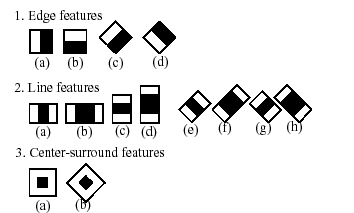
\includegraphics[width=3in]{img/haarfeatures.png}
\caption{A collection of Haar-like features used in the OpenCV implementation of a cascade classifier. These include the original features proposed by Viola-Jones \cite{viola2004robust} as well as additional features suggested by Lienhart et al. \cite{lienhart2002extended}. Image taken from the OpenCV site \cite{opencv2014cascade}.}
\label{fig:haar-features}
\end{figure}

The second component is to use the AdaBoost algorithm \cite{freund1996experiments} to create classifiers with high detection rates and low rejection rates \cite{bradski2008learning}. Each of these individual classifiers do not need to be accurate. The only requirement is that they are at least slightly better than random guessing. For this reason such classifiers are referred to in literature as weak learners. In the implementation presented in ref. \cite{viola2004robust} the AdaBoost algorithm is used both to select the best features and train the classifier. Each weak learner corresponds to a single feature perceptron. Feature selection is achieved through training a bunch of single feature classifiers on the data then selecting the best performing one and combining it with the previously selected classifiers. The data is then re-weighted using the errors in classification to give incorrectly classified examples a higher weighting and then retrained until the desired number of features are obtained.

The third component is to combine the weak classifiers into a cascade of classifiers, with the least complex classifiers at the beginning of the cascade and more complex ones at the end. This ensures that the majority of negative sub-windows are rejected early using classifiers that are quick to evaluate, but that later, more complex nodes in the cascade attempt minimise the occurrence of false positives. Once the cascade of classifiers has been trained it is very efficient to classify new examples by running the image through the cascade. AdaBoost is also used to train the classifier cascade. It achieves this by adding features to each level of the cascade until the desired rates of detection and false positives are met. Having more features at a later stage in the cascade means that the classifier will achieve higher detection rates and lower false positive weights but at the expense of extra computational time. In this way, classifiers at the start of the cascade will detect a high number false positives but will execute quickly and still remove a large number of irrelevant sub-windows. The following more complex set of features will reject many of the false positives from the previous layer and so on until a sub-window is either rejected or correctly detected as a face. 

The rest of this paper is dedicated to reviewing the performance of Viola-Jones object detection in various circumstances and discussing its application to the titular problem. Section \ref{sec:critique-of-method} reviews what problems Viola-Jones can be used to solve and what it cannot solve. Section \ref{sec:application-of-method} discusses how the technique could be applied to the titular problem and what the likely issues encountered would be. Section \ref{sec:conclusion} rounds off the the paper with conclusions drawn from the preceding sections. Finally, section \ref{sec:self-evaluation} provides my self evaluation of this paper.

\section{Critique of Method} \label{sec:critique-of-method}
Viola-Jones face detection represents a major breakthrough in the computer vision community through practical speed-ups, intelligent data structures, and clever use of the AdaBoost algorithm to make face detection in real time a possibility. However, success of the technique is not without its limitations and the technique has several possible failure modes.

At the time of publication of the technique had results that had ``detection and false positive rates which [were] equivalent to the best published results'' \cite{viola2004robust} but executed much more efficiently. Comparisons between the major approaches published at the time are given at the end of the paper, but the results are not entirely definitive due to most previous approaches not providing a full receiver operating characteristic (ROC) curves for their classifiers or did not publish their best results. In the case of Sung and Poggio \cite{sung1998example} only the MIT part of the common dataset was used (as the CMU dataset did not yet exist). In spite of this, the authors show that their technique provides roughly equivalent levels of performance given the available data. The authors also noted that the best performance was achieved using a voting regime between three classifiers trained with different negative examples, different negative vs. positive errors, and different criteria for also positives vs. classifier size.

Unfortunately the Viola-Jones has quite a few failure modes in which it will give a high number of either false positives or false negatives. One of the biggest drawbacks of the vanilla implementation presented in the paper is that it can only detect frontal images of faces. Faces viewed from the side won't be correctly detected by a detector trained on frontal face views. Likewise, training a face on both front and profile images will lead to a bad classifier because it cannot learn features important to both at once. The technique could be used to correctly detect faces viewed from the side by training a different classifier with sufficient positive and negative examples. Both sides of the face can then be accounted for by training a classifier for one side of the face, testing the image then flipping the image and running the classifier again to account for the other side. Similar problems occur when the classifier is presented with faces that are rotated, either in or out of the image plane. 

These problems are largely caused by the technique's dependence on such basic features. This leads to the classic time versus complexity trade off where in order for the algorithm to perform fast enough to run in real time, the features need to be quick to evaluate and therefore necessarily simple. This is also related to the concept that there is ``no free lunch'' in search and optimisation \cite{wolpert1997no}. The technique is very good under some circumstances but falls down in others. The basic set of features used by Viola-Jones are limited in the amount of domain knowledge they can encode in the learning procedure. The vertical and horizontal features fail to encode enough information about diagonal features, such as might be present in a face rotated 45 degrees out of the image plane. The detector finds side views particularly difficult to deal with because features presented in the diagonal appear less ``blocky'' which makes it more difficult for the detector to learn them \cite{bradski2008learning}. The simplicity of Haar-like features also makes the technique unsuitable to detecting objects that are not formed from distinct regular features, such as tree branches \cite{bradski2008learning}. Clearly two images of two different trees will show huge variation in branch position, size, colour etc. which Viola-Jones will be unable to generalise from. The features used will also cause issues when the shape of an object to be identified is itself the most distinguishing feature. The example given in ref. \cite{bradski2008learning} is a coffee mug. Colour, size, and decoration and orientation (e.g. location of the handle) of a mug can vary wildly between images, but the overal shape will remain the same.

\begin{figure}[!t]
\centering
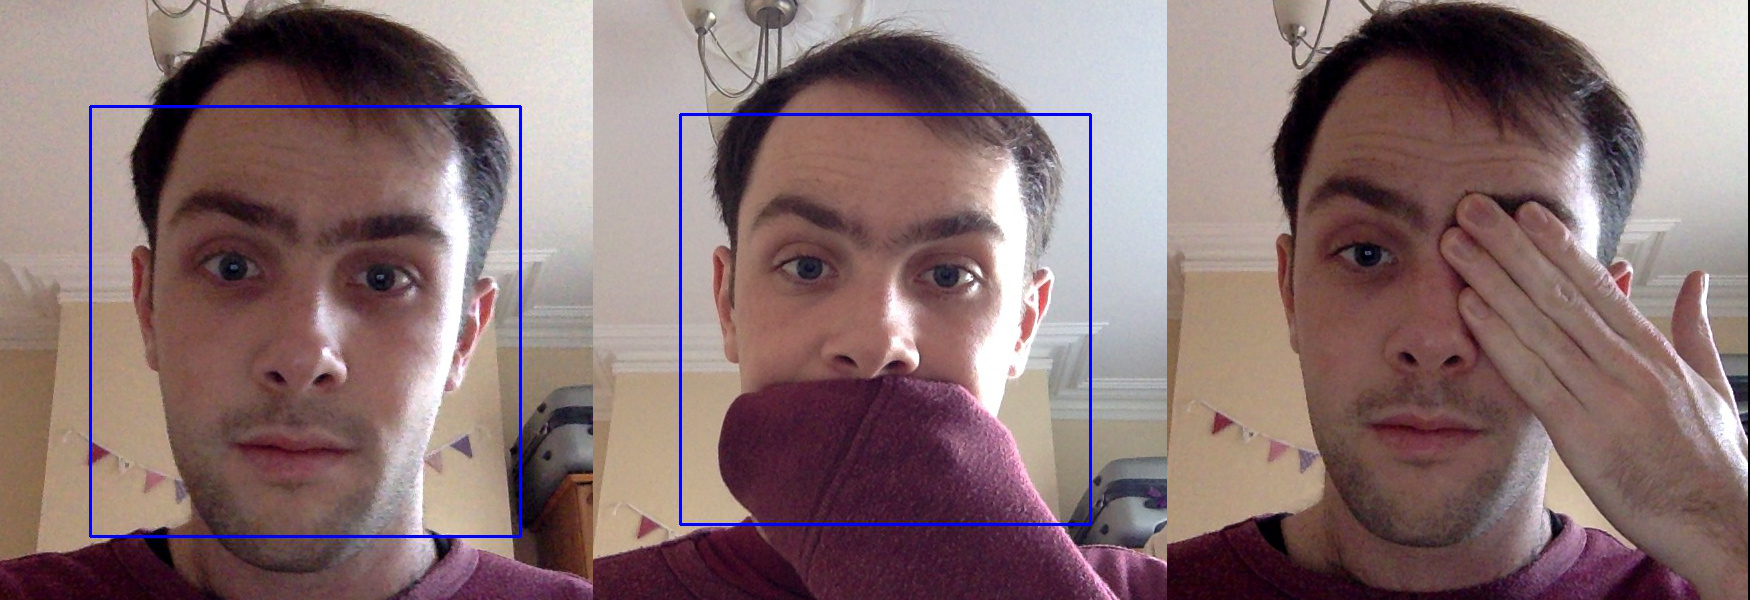
\includegraphics[width=3in]{img/face_detect_example.jpg}
\caption{Example of face detection using the Haar cascade in OpenCV. Occlusions of non essential areas (such as the mouth in the middle image) still result in a positive match, while occlusions of essential features such as the eyes or nose result in a false negative.}
\label{fig:occlusions}
\end{figure}

Jones and Viola \cite{jones2003fast} attempted to alleviate these issues by training multiple classifiers for each of the poses and using additional diagonal Haar like features. The choice of classifier used is decided using a decision tree. This gives a two step approach to classification in which the first step estimates the pose and the second runs the selected pose classifier. Further work by Lienhart et al. \cite{lienhart2002extended} provides empirical evidence that better results can be obtained from the Viola-Jones approach though the use of a number of extensions. They performed experiments with a broader set of Haar features which included rotated versions of the original features. These appeared to produce more accurate results despite complicating the learning procedure by successfully encoding more domain knowledge into the learning procedure that it would otherwise have difficulty learning. They also experimented with using small decision trees instead of decision stumps for weak classifiers. They suggested that this allows the weak classifier to learn dependencies between features which cannot be learned in a decision stump classifier. However, this obviously leads to an increase in the execution time as the complexity of the weak learners is increased.

Another key failure mode with the Viola-Jones algorithm is its robustness to occlusions. This largely depends on what is occluded in the image. The two key features identified during the training of the Viola-Jones technique show that a vertical rectangular feature over the nose and a horizontal rectangular feature over the eyes are the most important detection features for a face. This implies that Viola-Jones has some robustness against partial occlusions of non-essential areas (such as covering the mouth in the middle image of figure \ref{fig:occlusions}) and will still return a positive match. However, occlusions of prominent features used to classify a face will result in a false negative (such as occluding an eye in the right hand image of figure \ref{fig:occlusions}). Tweaking the parameters of the cascade can help to increase the detection rate of the occluded image, but this has the disadvantage of subsequently increasing the false positive rate. Lin et al. \cite{lin2004fast} have experimented with additional robustness against occlusions through by a two step process consisting of reinforcement training with bootstrapping and $k$-means clustering to reduce the false positive rate and training a selection of ``occlusion cascades'' which can be checked against when the regular cascade returns a negative match.

The success of the Haar cascade technique is also heavily affected by the quality of the dataset used during training. Careful preprocessing is required to ensure that all of the positive examples used in training are correctly aligned and are of a similar scale. A large number of negative examples also need to be prepared to provided sufficient training against false positives. However, it is also essential that the dataset used in training contains enough variance. As mentioned in section \ref{sec:introduction} human faces contain a large amount of variation. A good dataset should therefore capture a high amount of variation while still being well formed. In the dataset used in \cite{viola2004robust} used 4916 hand labelled images randomly taken from the web. These naturally contained a high degree of variation. Some examples had moustaches and facial hair, others had glasses or sunglasses. Different ethnicities and skin tone is included as re different lighting conditions. This subsequently leads to there being enough variation on the dataset to ensure that the classifier learns the common features shared between faces and therefore generalises well. A well formed data should contain examples where the object to be identified shows roughly the same feature set in every image and should only contain one view (such as the frontal view of a face) \cite{bradski2008learning}.

One final limitation with the Haar cascade method is the amount of time that it takes to train. This is not as much of a concern as other limitations because the important point about the Haar cascade approach is that once a classifier has been trained, it is fast enough to execute at frame rate. However, the original implementation of Viola-Jones took weeks to train. Exploitation of parallelism \cite{viola2004robust} and subsequent increases in computing power have brought the training time down, but training still remains a considerable task especially when this is combined with the amount of time required to pre-process a good dataset for use in training.

Despite these limitations the Haar cascade approach face detection remains one of the most popular approaches in the field. This is largely due to the fact that the method runs fast enough to be used at frame rate and therefore has a very wide variety of applications but does not need to sacrifice too much accuracy in order to achieve it. In summary the framework presented in ref. \cite{viola2004robust} is also not limited to the detection of faces. Relevant Haar features can be computed to be representative of a number of different objects, although the low complexity of these features restrict the classifier to working best with rigid body objects. The classifier also provides a small amount of robustness to partial occlusions of an object, but will fail if core features used in detection are occluded. A good dataset, with large quantities of both positive and negative examples, is required to effectively train a Haar cascade but providing  a decent dataset can be acquired the classifier will work well for many practical purposes.

\section{Application of Method} \label{sec:application-of-method}
This section analyses the potential suitability of applying the titular method to counting people. This is a very broad question the answer to which is largely dependant on the specifics of the application. Counting people is useful in a wide variety of circumstances. Safety applications are the among the most obvious. With automated people counting systems we could avoid disasters such as the one which occurred at the Hillsborough stadium in 1989. Customer service and management is another practical use for such a system. Knowing how many people are queueing at a checkout and alerting management to open another would be lead to more efficient management of people. Such a system would also have financial relevance, such as counting attendance to an event and making sure everyone has paid. An essential realisation is that counting people in a scene using an approach based on the Viola-Jones technique boils down to a person detection problem. If people in a given scene can be reliably detected independently from one another then they can be counted.

What components are required for a people counting system? One of the most obvious requirements is that it needs to be accurate. How accurate is ``good enough'' is dependant on the system implementation. In the case of preventing overcrowding in a stadium the number of people counted does not have to be exact, so long as a good enough estimate is achieved to know when an area is becoming over crowded. In a system that is counting people in order to charge the correct amount you would need an exact and accurate count so that customers are charged the correct price. A customer service scenario would probably demand a less accurate approximation but would still need to be accurate enough to be useful. Another key factor would be the system's robustness. Groups and crowds of people are a constantly changing and dynamic thing to monitor. Given a typical image of a group of people there is likely to be a large amount of variance between people in the scene, including their height, body size, clothes etc. Partial or total occlusions are also highly likely especially in very crowded scenes or constantly changing scenes (such as a street scene where cars are constantly passing). A successful people counter needs to be able to handle a high degree of variance in a scene as well as have some robustness against partial and total occlusions in order to be accurate enough for practical purposes. Finally, the system will most likely need to be fast. While there are likely to be circumstances where the a people counting system is useful without running in real time, the most interesting practical applications of such a system require that it operates at frame rate. Finding out that a stadium is overcrowded is useless thirty minutes after the event.

The practical limitations of a Haar cascade causes some immediate issues when compared with the requirements for a people counter. As mentioned in the preceding section, the basic implementation of a Haar cascade outlined in ref. \cite{viola2004robust} uses only very basic rectangular features classify a face from the frontal position. This works well because even though there is a high degree of variance between faces almost all faces share a common structure and it is assumed that the faces to be detected will be viewed from a frontal position. These two assumptions cannot be used when applying the technique to counting people in a scene. Obviously in a real world scene it is unlikely that all of the people in a scene will be facing directly at the camera. This could be the case for some uses, for example if the application was counting people in planned photographs such as wedding photos, but this is probably not the case. A modified Haar cascade that has some robustness to rotations such as ref. \cite{jones2003fast} could help, but what about situations where there are no clear faces, such as people viewed from behind? Or people with hoods up and not looking towards the camera?

This suggests a classifier should be trained to detect bodies and not faces in a scene. While faces are not guaranteed to be reliably available in a scene, images of human bodies almost certainly will be. However, training a classifier to detect human bodies poses its own assortment of issues. With faces, each face typically has a nose in the centre and a set of eyes positioned horizontally above the nose. This gives a common element between all faces that a classifier that uses rigid rectangular features such as the original implementation of a Haar classifier can be trained to detect. Human bodies on the other hand are much less rigid in there appearance. While human bodies share a degree of similarity (two arms, two legs, one torso etc.) each of these independent parts can the move independently, making the overall structure of a human body far more fluid than the structure of a face. The orientation problem is also exacerbated further when training a body detector over a face detector. A typical street scene will show people from all different angles. They may be viewed from in front, behind, or in profile. They may also be standing, sitting, or laying down. Occlusions will still be a problem for a body classifier. A classifier is trained to detector the common features of a body (such as a torso) and these features become obscured (such as another person walking in front) the classifier will fail.

However, despite these issues there is still hope for the application of the technique the problem in question. Viola et al. have themselves carried out experiments adapting the Haar cascade to the practical application of detecting pedestrians \cite{viola2003detecting}. In their approach they modify the approach take in ref. \cite{viola2004robust} to include an additional set of diagonally shaped features. This is to try and capture some domain knowledge about diagonal shapes within an example. They also realised that motion between two frames of video can encode information about whether a section of a scene contains a pedestrian. Using this they created filters which operate on the absolute difference between the two frames shifted in different directions. The Haar like features can still be computed using the integral image representation on the different images. While this approach is shown in the paper to produce decent results approach it assumes that people are moving in the scene. If a person stops moving then the classifier will fail to find them as the difference between the images will likely be too minimal. 

Garcia et al. \cite{garcia2008effective} experimented with vanilla Viola-Jones in combination with background subtraction to try and focus the classifier on certain areas in the scene. Their work found poor performance due to the crowdedness and illumination conditions of their real world dataset. They concluded that a density estimation approach yielded much more positive results. Density estimate approaches have the advantage that they make no assumptions about the features, orientation or motion of people in a scene (which is effectively the inductive bias of Viola-Jones). In ref. \cite{garcia2008effective} the only assumptions were that the background could be successfully extracted and everything in the foreground is a person. The method used in ref. \cite{garcia2008effective} also had some invariance to objects in the foreground that were not human, such as pets or luggage. Another approach is to train a classifier to detect the heads of people. This is exactly the approach taken by Subburaman et al. \cite{subburaman2012counting} with their head counting approach to counting people in crowded scenes. This has particular relevance if the target application is in crowded areas where it is likely that the majority of a persons body is occluded by other people in the scene. To help aid the classifier they use a gradient based approach to find regions of interest before applying the classifier. Yet another approach to the problem of human detection has been presented by Mikolajczyk et al. \cite{mikolajczyk2004human} which attempts to produce a human detector using a combination of 7 different invariant body parts such as different orientations of the face, head, upper and lower body and combining them using a probabilistic model for the joint co-occurrence of features. This obviously takes into consideration issues with variance in the positioning of human body parts by modelling each part independently and then using proximity information boost the accuracy of a prediction.

An additional source of information that could be used to extend the accuracy of a Haar cascade based people counter is the use of multiple cameras. Viewing a scene from multiple angle adds additional complexity to the system because the views from each of the cameras need to be correlated in order to avoid counting some people twice. The advantage of multiple cameras is that this allows you to utilise multiple sources of information. Using this as part of a voting system can help with resolving an ambiguous detection from a single detector and prevent problems with occlusions. Multiple cameras mean that people who might be difficult to detect from one view are easier to spot from another angle. Zhang et al. \cite{zhang2006robust} proposed a multi-view face detection system that used an AdaBoost variant FloatBoost \cite{li2004floatboost}.

Putting all of these points together it becomes clear that the Viola-Jones method is not enough on its own to produce a system that will be accurate enough for practical purposes in the real world. Weighing the different sources listed in this section suggests a number of improvements that could be undertaken to try and make Viola-Jones applicable to real world people counting. The first extension required for a practical people counting system using Viola-Jones would be to extend the feature set used to include features such as those suggested by Lienhart et al. \cite{lienhart2002extended}, or if the system is going to be used in a scenario where people are likely to be moving around a lot, by using motion features like those suggested by Viola and Jones in ref. \cite{viola2003detecting}. This would make the classifier more robust to real world circumstances where people are unlikely to be directly looking at the camera and will have different poses and rotations in and out of the image plane. Multiple classifiers could also be used. For example, one could be trained to detect a face in the frontal position, while another could detect the side of a face (and the image flipped to detect the other side). 

Whether the classifier used would be trained to detect a face or a the whole body largely depends on the target application of the system. If the system is going to be used in an application with a relatively sparse count of people in the scene then training a body or invariant body parts classifier seems to be the correct method to use, particularly if the subjects are likely to be moving across a range of frames. However, in crowded scenes a whole body detector isn't likely to work as only the very top of a person such as their head is likely to be visible to the camera. In this case it would be better to train a classifier to detect just the head. However, as shown by Garcia et al. \cite{garcia2008effective} this generally performs worse than other methods. Multiple cameras could be used to gain a better perspective on a scene and give some additional information that would catch missed people due to occlusions. The part of a human that the classifier is trained to detect is also reliant on positioning of the camera within the system. For example, a frontal face detector is not going to work very well if the camera is necessarily positioned side onwards to the flow of people through an area. However, the choice of the camera position can be advantageous to the implementation of a people counting system. For example, if the proposed system was supposed to count the number of people in a line at a checkout, it may be better to position the camera side on to the checkout so that the queue of people appear side on to the camera. That way people are not occluding each other as they stand in a line at the checkout.

Depending on the power of the architecture of the equipment to be used in the counting system, the research in this paper suggests that it would be advantageous to utilise multiple classifiers for different likely scenarios in the scene. For example, Lin et al. \cite{lin2004fast} showed that they could using multiple classifiers could improve robustness by training separate classifiers that deal with occlusions or the work by Jones and Viola \cite{jones2003fast} which uses different detectors for each pose. Obviously using multiple classifiers adds to the computational complexity of the system and depending on the hardware requirements of a people counting system it may be infeasible if the the equipment has low processing power and the system is required to run at frame rate. Of course this might not be such an issue if the system is not required to run at frame rate or the machine doing the analysis is powerful enough to handle it.

Another hardware consideration would be the use of a thermographic camera to help narrow the search space of by thresholding everything in the original image that does not correspond to a strong enough heat signature in the thermal image, thus focussing the detector. This would provide an advantage over other background subtraction techniques in that it would remove anything that isn't hot (such as furniture). Depending on the environment this could drastically reduce the search space. Obviously things other than people are hot in the real world which would cause this approach to be less useful. Also in a scene which mostly consists of crowds the thermal camera may be overloaded with too much information. Yet another issue would be the additional complexity of computing a homography to map the capture from the thermal camera to the regular camera. Despite the author's best efforts no relevant sources could be found to support or refute this idea.


% An example of a floating figure using the graphicx package.
% Note that \label must occur AFTER (or within) \caption.
% For figures, \caption should occur after the \includegraphics.
% Note that IEEEtran v1.7 and later has special internal code that
% is designed to preserve the operation of \label within \caption
% even when the captionsoff option is in effect. However, because
% of issues like this, it may be the safest practice to put all your
% \label just after \caption rather than within \caption{}.
%
% Reminder: the "draftcls" or "draftclsnofoot", not "draft", class
% option should be used if it is desired that the figures are to be
% displayed while in draft mode.
%
%\begin{figure}[!t]
%\centering
%\includegraphics[width=2.5in]{myfigure}
% where an .eps filename suffix will be assumed under latex, 
% and a .pdf suffix will be assumed for pdflatex; or what has been declared
% via \DeclareGraphicsExtensions.
%\caption{Simulation Results}
%\label{fig_sim}
%\end{figure}

% Note that IEEE typically puts floats only at the top, even when this
% results in a large percentage of a column being occupied by floats.


% An example of a double column floating figure using two subfigures.
% (The subfig.sty package must be loaded for this to work.)
% The subfigure \label commands are set within each subfloat command, the
% \label for the overall figure must come after \caption.
% \hfil must be used as a separator to get equal spacing.
% The subfigure.sty package works much the same way, except \subfigure is
% used instead of \subfloat.
%
%\begin{figure*}[!t]
%\centerline{\subfloat[Case I]\includegraphics[width=2.5in]{subfigcase1}%
%\label{fig_first_case}}
%\hfil
%\subfloat[Case II]{\includegraphics[width=2.5in]{subfigcase2}%
%\label{fig_second_case}}}
%\caption{Simulation results}
%\label{fig_sim}
%\end{figure*}
%
% Note that often IEEE papers with subfigures do not employ subfigure
% captions (using the optional argument to \subfloat), but instead will
% reference/describe all of them (a), (b), etc., within the main caption.


% An example of a floating table. Note that, for IEEE style tables, the 
% \caption command should come BEFORE the table. Table text will default to
% \footnotesize as IEEE normally uses this smaller font for tables.
% The \label must come after \caption as always.
%
%\begin{table}[!t]
%% increase table row spacing, adjust to taste
%\renewcommand{\arraystretch}{1.3}
% if using array.sty, it might be a good idea to tweak the value of
% \extrarowheight as needed to properly center the text within the cells
%\caption{An Example of a Table}
%\label{table_example}
%\centering
%% Some packages, such as MDW tools, offer better commands for making tables
%% than the plain LaTeX2e tabular which is used here.
%\begin{tabular}{|c||c|}
%\hline
%One & Two\\
%\hline
%Three & Four\\
%\hline
%\end{tabular}
%\end{table}


% Note that IEEE does not put floats in the very first column - or typically
% anywhere on the first page for that matter. Also, in-text middle ("here")
% positioning is not used. Most IEEE journals/conferences use top floats
% exclusively. Note that, LaTeX2e, unlike IEEE journals/conferences, places
% footnotes above bottom floats. This can be corrected via the \fnbelowfloat
% command of the stfloats package.



\section{Conclusion} \label{sec:conclusion}
In conclusion, the first half of this paper has presented a review of the highly susccessfully Viola-Jones approach to face detection and discussed subsequent work building upon the basic implementation of the framework to include new features and enhanced set-ups for different problem domains. The Haar cascade has a wide number of applications a variety of different to object detection problems and is in no way limited to the just face detection. The key insight that the Viola-Jones object detection framework brings to the table are speed-ups allowing technology from the early 21$^{st}$ century to perform object detection at frame rate. The first key contribution from the technique was the use of the integral image data structure to reduce the time complexity of evaluating features to a constant time operation. The second contribution was the use of the AdaBoost algorithm to perform feature selection of Haar like features which can be evaluated using the integral image. Finally they presented a way to combine classifiers into a degenerate decision tree with successively more complex nodes called a classifier cascade. These three contributions produced a framework that was extremely efficient yet very accurate at detecting rigid body objects with ``blocky'', largely invariant features.

The second half has focused on the application of the Viola-Jones framework and the subsequent work and variants to the titular question of counting people. We have suggested that the Viola-Jones framework presented in its most basic form would not be robust enough to be used practically as part of a useful people counting system unless such a system was used in a highly unrealistic environment. We have also presented a selection of existing work carried out in the field since the Viola-Jones break through with various extensions on the original framework. Combining the major findings of the approaches we have suggested what modifications work probably be desirable to a system wishing to use Viola-Jones for counting people, while keeping a open mind to the broadness of the titular question. We have concluded in that for practical use in people counting a Viola-Jones based system would need to boost its robustness against the high degree of variance in the pose of bodies and face among real life scenes. This would most likely involve adding new features that capture a greater amount of domain knowledge such as diagonal shapes \cite{lienhart2002extended}, or features present in the motion of pedestrians \cite{viola2003detecting}. Such a system would also need to consider the high degree of occlusions likely to be present in a real world scenario and take advantage of either a multi-detector or multi-camera approach. Either approach would be able to add support to deal with occlusions of essential features that cannot be handled by the vanilla Viola-Jones technique alone. However, due to the instability of the framework in real life systems due to the high amount of variance in a typical scene and the framework's lack of robustness thanks to it's necessarily simple features an alternate approach based on the methods such as density estimation which do not make assumptions about position or pose may yield better results in a practical setting and would be an interesting area for further experimentation.

\section{Self-Evaluation} \label{sec:self-evaluation}
I believe that this piece of work is worth an A- as defined by table 2 in section 5.7 of the Aberystwyth University student handbook. I believe that this would be a balanced choice based on the work presented in this document and on what I would do differently with hindsight. I think I deserve this grade because I have demonstrated that I have read and understood the paper upon which this assignment is based. I have also clearly analysed the major success and failure methods of the technique under examination and outlined why the technique was such a breakthrough in the computer vision field. In the second section I have researched a variety of existing work in the area of detecting people using the Viola-Jones technique and drawn conclusions based on these sources. I feel that I have achieved this fairly successfully and that I have shown I can read a comment on scientific research. I have also shown that I can propose reasonable suggestions on how to implement the system proposed in the scenario. However, there is always room for improvement. I found the amount of background reading and how to write about it effectively one of the biggest challenges and I feel that there are some areas which I could have expanded on further. In hindsight I would have written more in comparison with alternative approaches used to count people using computer vision and focused less on extensions of Viola-Jones. I could of also possibly expanded the application section with some more outlandish suggestions than I listed here. I also feel that I could have played with the detector more in OpenCV and perhaps have trained my own classifier on some pedestrian data and included some actual performance results for the vanilla Viola-Jones implementation. Finally, I feel I could of written a better description of how the technique works. I found it difficult to explain concisely as the system is fairly complex and accurately describing how each component hangs together was challenging.

% conference papers do not normally have an appendix

% trigger a \newpage just before the given reference
% number - used to balance the columns on the last page
% adjust value as needed - may need to be readjusted if
% the document is modified later
%\IEEEtriggeratref{8}
% The "triggered" command can be changed if desired:
%\IEEEtriggercmd{\enlargethispage{-5in}}

% references section

% can use a bibliography generated by BibTeX as a .bbl file
% BibTeX documentation can be easily obtained at:
% http://www.ctan.org/tex-archive/biblio/bibtex/contrib/doc/
% The IEEEtran BibTeX style support page is at:
% http://www.michaelshell.org/tex/ieeetran/bibtex/
%\bibliographystyle{IEEEtran}
% argument is your BibTeX string definitions and bibliography database(s)
%\bibliography{IEEEabrv,../bib/paper}
%
% <OR> manually copy in the resultant .bbl file
% set second argument of \begin to the\textsl{•} number of references
% (used to reserve space for the reference number labels box)
\bibliographystyle{IEEEtran}
\bibliography{references}

% that's all folks
\end{document}


